\documentclass{article}\usepackage[]{graphicx}\usepackage[]{color}

\usepackage{alltt}
\usepackage{float}
\usepackage{graphicx}
\usepackage{tabularx}
\usepackage{siunitx}
\usepackage{amssymb} % for math symbols
\usepackage{amsmath} % for aligning equations
\usepackage{textcomp}
\usepackage{booktabs}
\usepackage{mdframed}
\usepackage{natbib}
\usepackage{comment}
\usepackage{booktabs}
\usepackage[colorinlistoftodos]{todonotes} % to make comments on the margin
\usepackage[small]{caption}
\setlength{\captionmargin}{30pt}
\setlength{\abovecaptionskip}{0pt}
\setlength{\belowcaptionskip}{10pt}
\topmargin -1.5cm        
\oddsidemargin -0.04cm   
\evensidemargin -0.04cm
\textwidth 16.59cm
\textheight 21.94cm 
%\pagestyle{empty} %comment if want page numbers
\parskip 7.2pt
\renewcommand{\baselinestretch}{1.5}
\parindent 0pt
%\usepackage{lineno}
%\linenumbers

%% R Script

\title{Unravelling the phenology-phylogeny tangle.}

% alternative titles:
%% An expanded bayesian phylogenetic mixed model to unravel the phenology-phylogeny tangle. %% this sounds too methodsy

\begin{document}

\maketitle

\noindent Authors:\\
The Wolkovich Lab in 2019 \& collaborators $^{1,2,3,4}$ % Will Pearse, Jonathan Davies also
\vspace{2ex}\\
\emph{Author affiliations:}\\
$^{1}$Forest \& Conservation Sciences, Faculty of Forestry, University of British Columbia, 2424 Main Mall, Vancouver, BC V6T 1Z4;\\
$^{2}$Arnold Arboretum of Harvard University, 1300 Centre Street, Boston, Massachusetts, USA;\\
$^{3}$Organismic \& Evolutionary Biology, Harvard University, 26 Oxford Street, Cambridge, Massachusetts, USA;\\
$^{4}$Edificio Ciencias, Campus Universitario 28805 Alcalá de Henares, Madrid, Spain\\
 

\vspace{2ex}
$^*$Corresponding author: ignacio.moralesc@uah.es\\
\renewcommand{\thetable}{\arabic{table}}
\renewcommand{\thefigure}{\arabic{figure}}
\renewcommand{\labelitemi}{$-$}
\setkeys{Gin}{width=0.8\textwidth}

%%%%%%%%%%%%%%%%%%%%%%%%%%%%%%%%%%%%%%%%%%%%%%%
%%%%%%%%%%%%%%%%%%%%%%%%%%%%%%%%%%%%%%%%%%%%%%%
\clearpage

\begin{comment}
\section*{Rationale \& Significance}

Previous work has looked at the phylogenetic conservatism of phenology across plant species, finding that, first flowering is significantly conserved \citep{davies2013phylogenetic} and, when using OU models so are shifts in first flowering and the slopes of the relationship between flowering and year \citep{rafferty2017global}. Research in this area has focused on the phenotype (phenological event or its shifts) rather than on the cues---i.e. how shifts in the environment trigger species responses. Beyond whether or not phenology is phylogenetically conserved, determining evolutionary constraints in phenological responses to temperature and daylight, may have deeper implications for forecasting under ongoing change.\\ 

Nevertheless, previous work on the phylogenetic conservatism of phenology has still not addressed:\\

- Emphasis has been put on the phenotype rather than on the cues\\
- Are phenological responses in lab experiments conserved as well? In \cite{joly2019importance} the authors check this with a focus on intraspecific variations\\
- How the sensitivities to different environmental cues are conserved?\\
- Are the responses to certain cues more strongly conserved than to others?\\
- How does accounting for phylogeny affects model estimations of cue sensitivity?\\

And beyond work on phylogenetic conservatisms, previous comparative research on phenological responses to cues (experimental or observational) has either:\\

- Ignored phylogenetic relationships (or the fact that species are not independent units)\\
- Accounted for phylogenetic relationships assuming that they are \emph{stationary} across predictors-traits and can be modelled by including phylogenetic Variance-Covariance in model residuals. This is the rationale behind common-use PGLS approaches but it \"hides\" the partial phylogenetic constraints to model predictors.\\ 

An overlooked question so far is whether we could gain any additional information by accounting for independent phylogenetic structuring in each species responses to each predictor in a multi-linear response model setting. Typical methods are good to account for species non-independence but provide little insight relative to phylogenetic effects on each predictor.
\todo{I think the new approach is a bit of a game changer as it shifts the focus from empirical results of phylo-constrains on phenology to a more methodsy paper. We need to decide a focus.}



The potential interest of findings in this direction stem from:\\
- better predictions of phenology (or need to account for it in models)\\
- better understanding of the mechanistic basis of plant responses to climate\\
- better design the next generation of experiments \\


## bits from previous version of the abstract to remove at a later stage

The plasticity of these responses may ultimately determine species ability to withstand ongoing environmental change because non-plastic species may undergo developmental events under unadequate conditions---e.g. a species advancing flowering too much could see increased the risk of frost events. Phenology describes the responses to seasonal change in environmental cues and while it is often regarded to as a rather plastic trait, it is still unknown whether or not phenology is a phylogenetically conserved trait. 


\end{comment}

\section*{Abstract}

Plants have evolved responses to environmental cues able to inform them about the temporal distribution of key resources---i.e. energy and light. The responses to individual cues such as forcing (or spring warming) have shown to be subjected to some degree of evolutionary conservatism. Yet, plants do not respond to isolated cues but to a combination of interacting cues, which difficults accurate predictions of phenology in the face of environmental change. Whether and how evolution has constrained phenological responses to combinations of interacting cues is not yet understood even when this knowledge could enhance model predictions and inform how different plant lineages have adapted to environmental change along their evolutionary histories. Here we use Bayesian hierarchical models and the most complete dataset on tree species phenological responses measured in experimental conditions to: (a) test if phenological responses to three major interacting cues are conserved phylogenetically when considered jointly, (b) compare the phylogenetic signal in the responses to different cues and, (c) test whether coefficient estimates differ between models assuming phylogenetic independence among species and models that explicitly incorporate phylogeny. Results show non-random phylogenetic structuring of phenological responses, highly variable across species and cues. More interestingly, regression coefficients shift when models control for phylogenetic effects, particularly so for forcing, which becomes the most important cue. Taken together, our results suggest that phylogeny should be incorporated into studies modelling multi-species phenological responses, as such responses have been jointly constrained through evolution and thus are not independent.  


\begin{comment}
\begin{enumerate}
\begin{enumerate}
\item How plants respond to environmental cues--i.e. temperature, daylight--may determine their resilience or vulnerability to ongoing climate change. 
\item Phenology provides a good description of plant responses to to the environment. 
\item Phenology has been regarded to as a rather plastic trait, thus with a lot of variation both intra- and inter-specifically.
\item Variation in phenology could have randomly accummulated across species (and then phenology would be an evolutionary labile trait), or be structured in the phylogeny so that closely related species resemble more each other in their phenological responses (conserved trait).
\item Whether or not phenology is conserved has implications for the need to account for phylogenetic autocorrelation in cross-species analyses.
\item More interestingly, given that phylogeny can act as a proxy for other (unaccounted) traits that may be linked to phenology, including it in models could lead to more accurate predictions.
\item Here we use Bayesian hierarchical models and the most complete dataset on tree species phenological responses measured in experimental conditions to: (a) test if tree species responses to cues are conserved phylogenetically, (b) compare the phylogenetic signal in the responses to different cues and, (c) test the abiltiy of phylogenetically informed models to improve predictive accuracy of phenology.
\item Results show non-random phylogenetic structuring of phenological responses, highly variable across cues.  
\item Taken together, our results suggest that phylogeny should be incorporated into studies modelling multi-species phenological responses, as such responses have been constrained through evolution and thus are not independent.  
\end{enumerate}
\end{comment}

% not yet satisfied about the pitch - this is already said in Davies et al. 2013 
% should we emphasize the fact that we are using experimental/lab data? What are the gains with respect data from the field?

% we need an angle of at least some novelty

%%%%%%%%%%%%%%%%%%%%%%%%%%%%%%%
% Introduction
%%%%%%%%%%%%%%%%%%%%%%%%%%%%%%%
% Meeting call notes: https://github.com/lizzieinvancouver/ospree/wiki/Phylogeny-and-phenology


\section*{Introduction}

\begin{comment}
\begin{enumerate}
\item Predicting species responses to recent anthropogenic climate change presents a major challenge to ecological forecasting
\begin{enumerate}
\item On average global temperatures are warming, but there is regional and seasonal variation behind this average and shifts along other climate axes such as precipitaion are more complex than simple increases % or  but climate change is atcually multivariate and complex
\item Over the past few decades empical studies have suggested that plants are shifting in their geographical distributions, moving to more northern latitudes and elevations, and shifting the timing of their life cycles
\item However, responses are highly variable across species.
\item Understanding how different species lineages have evolved their phenotypic responses to the combined effects of environmental change would greatly aid prediction
\end{enumerate}
\end{comment}
Forecasting remains a major challenge in ecology, especially as anthropogenic climate change drives demand for more accurate forecasts across species. As global temperatures warm, plant species are shifting the timing of their life cycles \citep{Cleland:2007or} and their geographical distributions towards higher latitudes and altitudes \citep{chen2011}, but responses are highly variable across species \citep{menzel2020}. Some of this variability is due to the complexity of climate change itself---the regional and seasonal variation in warming underlying average trends and shifts in other climate axes (e.g. precipitation)---however, much of it is driven by species-specific variation in response to environmental change, which we can only predict for a few well-studied species. More accurate forecasts will require efforts to scale our understanding across more plant species. Understanding how different plant lineages have evolved their phenotypic responses to the combined effects of multiple dimensions of environmental change would greatly aid prediction.\\ %the last sentence feels a bit general still - try better connection with next paragraph

\begin{comment}
\item Environmental cues matter as they inform organisms about the temporal distribution of key resources.
% Understanding how different plant lineages have evolved their phenotypic responses to the joint effects of interacting environmental cues remains a challenge. % Lizzie says: I like this, but the introduce of cues and lineages at once feels too much at the very start... suggested alternative intro, but take or leave what works!
\begin{enumerate}
\item Responses (and their evolution) to cues are usually studied individually assuming that a given phenotypic response (e.g. time of leafout) is linked to a single cue, when likely multiple ones operate interactively (and have done so across evolutionary history) to shape that response. 
\item For example, light, nutrients and water often determine growth rates and size
\item Or how the timing of many recurring life cycle events (phenology) is determined by a combination of temperature and light. 
\end{enumerate}
\end{comment}
Decades of research show that plants use environmental cues to time their phenotypic responses with the temporal distribution of key resources and to avoid periods of high abiotic or biotic stress \citep{larcher1980,Chuine2000}. Commonly, responses to environmental cues, and their evolution, are studied individually, assuming that a given phenotypic response is predominantly linked to a single cue: for example, that time of leafout is driven by summed heat during early spring \citep{Wolkovich:2012n,davies2013phylogenetic}. Such efforts ignore a more likely scenario for most phenotypic traits where multiple cues interacting along evolutionary history have shaped plant responses \citep{}. For example, species-level growth rates or plant height may be determined by the interaction among several cues---e.g. soil nutrients, water availability and light \citep{larcher1980}. Similarly, the timing of recurring life cycle events (phenology) is determined by a combination of temperature and light \citep{chuinearees}.\\

\begin{comment}
\item Phenology makes for an ideal study case of species' responses to interacting environmental cues.
\begin{enumerate}
\item Phenology is a critical trait to studying biological responses to climate change.
\item In temperate species its cue system is generally known: forcing, chiling, photoperiod
\item It is amongst the few phenotypic characters (if any other exists) for which there are multi-species experimental data on its responses to the three major environmental cues. 
\item Out of these three major cues that affect plants, few multi-species analyses have considered all three simultaneously, with repeated consensus that chilling and forcing would prevail, but would this pattern hold if evolution/phylogeny was accounted for? % or perhaps avoid talking about phenology yet and making this opening more general about traits and phenotypes and their response to cues: from Lizzie's notes: the trait is a phenotype itself is made of underlying traits that respond to different cues. (For example, plant height or growth is a function of responses to water and nutrients.)
 \end{enumerate}
% My suggestion is a paragraph on a pheno by phylo, then one one on phylo methods (short), but you could have an additional paragraph on more pheno x phylo, see commented out chunk below
\end{comment}
Phenology may provide an ideal case study to gain insights on how species responses to interacting environmental cues have evolved because the basic cue system is well established \citep{chuinearees}. In temperate plants, phenology is generally determined by forcing---warm temperatures during the growing season, chilling---cool temperatures during dormancy period over winter, and photoperiod \citep{chuinearees}. Further, phenology is one of few phenotypic traits where decades of research provide multi-species experimental data on plant responses to these three major cues. Recent multi-species analyses considering forcing, chilling and photoperiod have shown that chilling and forcing together determine complex non-linear responses to warming \citep{flynn2018,ettinger2020}, complicating forecasting. In addition, studies found remarkable variation across species in their responses to cues, raising the question of whether such variation is phylogenetically structured. If phylogenetically close species have evolved similar responses to cues it could facilitate forecasting to unmeasured species, and provide insights into how cues have evolved in the past. \\

\begin{comment}
\item Phenology x phylogeny quick review ...
\begin{enumerate}
\item It is evolutionary conserved (to some extent, review antecedents).
\item Research in this area has focused on the phenotype (phenological event or its shifts) rather than on the cues---i.e. how shifts in the environment trigger species responses. For example, first flowering is significantly conserved \citep{davies2013phylogenetic}. 
\item Whether shifts in first flowering over time are also conserved is less clear and all inference to date is based on observational data, where geographical signals in phylogeny may drive trends attributed to phenology \citep[e.g.,][]{rafferty2017global}, as discussed in \citep{davies2013phylogenetic}. % This Rafferty paper is so flawed analytically that I suggest we better couch how we cite it ... see what you think... could also check Pearse NEE paper for how phylogeny affected answers
\item Further, additional questions remain open: in a multi-species context, have specific lineages adapted more strongly to some of the cues? or to any combination of cues? Is there any cue that is particularly labile?
\item Answering these questions may: (i) inform about the need to account for phylogeny in phenological models and predictions, and (ii) expand our knowledge on how phenological responses have been constrained so far, which would be relevant in a context where species' sensitivities to warming temperatures seem to decline.  % And extend to other responses to global change?
\end{enumerate}
\end{comment}
Accummulating literature on the evolutionary constraints of phenological responses to cues suggests that phenology is phylogenetically conserved, at least to some extent \citep{davies2013phylogenetic}. For example, dates of budburst, leafout or first flowering, and shifts in these dates in response to warming are significantly conserved \citep{davies2013phylogenetic,joly2019importance}, as are traits correlated with phenology, such as seed size \citep{bolmgren2008time,willis2008phylogenetic}. Almost all of this literature has focused on the phenotype, which may be more strongly determined by the local environment (e.g., the climate where phenology was measured), rather than species' intrinsic responses to the environment through time \citep[but see][]{}. And out of the few studies looking at phylogenetic structuring of responses to cues, the typical focus is on one single cue \citep{}, even if the evolution of responses to one environmental cue would have not occurred in isolation from the influence of others. 
% EMW (26Feb2022): Not sure what refs you're thinking of here ... in the two citep above: I feel like all studies beyond the Joly one are using observational data and some form of spring temp, which feels like one cue. Let me know what you're thinking and I can help with citations and language. 
Tackling the evolutionary constraints of phenological responses to multiple cues simultaneously would allow answering questions such as: have specific lineages adapted more strongly to some of the cues or to any combination of cues? Is there any cue that is particularly labile? These questions are highly relevant because answering them would (i) inform about the need to account for phylogeny in phenological models and predictions, and (ii) expand our knowledge on how phenological responses have been constrained so far, which would be relevant in a context where species' sensitivities to warming temperatures seem to decline.\\ % And extend to other responses to global change? -nacho: not sure how to include this. Also, the paragraph needs work as it reads perhaps a bit long and ranty.



\begin{comment}
\item Current methods advanced our understanding of how specific lineages have adapted phenotypic responses to the environment, but don't capture the complexity of responses that depend on interacting environmental cues. 
\begin{enumerate}
\item Traditional phylogentic comparative methods (such as PGLS) allow us to fit models to species phenotypic traits while correcting for the non-independence among species.  % Add cite and text to Revell's 2010 paper here OR in methods
\item But they do not allow the response to environmental cues to evolve over time while operating in concert with other cues. % the response have been constrained through evolution 
\item However, exploratory methods show that responses can shift dramatically across a phylogenetic  \citep{davies2019phylogenetically}
% I moved a chunk here down to methods ... I would keep this above section relatively short and save some of this for methods and some for discussion
\end{enumerate} 
\item Here, we expand previous phylogenetic regression settings to explicitly estimate phylogenetic constraints on the interactions among predictors (cues). 
\begin{enumerate}
\item Common phylogenetic regression accounts for phylogenetic relationships as a grouping factor either explicitly (PMM) or implicitly (PGLS). Here we present one possible approach that accounts for more complex interactions going on among predictors, which would be reflected in the species-level slopes being allowed to vary as a function of the phylogeny, rather than keeping slopes constant and only allowing the intercepts (or residuals) to vary. 
\item We ignore whether this is important and maybe current models are fine. 
\item In a first attempt at establishing whether or not it is important, we compare results from a common hierarchical model with partial pooling on the slopes that does not allow for phylogenetic constraints to affect slope estimates against results from a phylogenetic hierarchical model allowing phylogeny to constrain partially pooled slopes. %% this needs rephrasing!!!
\item We do so for an unprecedented dataset on phenological responses to environmental cues determined experimentally. 
% \item This is one possible approach but there may be alternative ones. % Skip saying there may be others and I moved up first part ... 
\end{enumerate}
\end{comment}
While current methods have advanced much of our understanding of how specific lineages adapted phenotypic responses to the environment, they were not originally designed to capture the complexity of phenotypes evolved in response to multiple interacting cues. For example, typical phylogenetic regression accounts for phylogenetic relationships as a grouping factor either explicitly (Phylogenetic Mixed Model; \cite{housworth2004phylogenetic}) or implicitly (Phylogenetic Generalized Linear Models; \cite{revell2010phylogenetic}), assuming all phylogenetic structuring to only affect model intercepts (or residuals). This assumption is known to be little reallistic, particularly in presence of type II error hidden by markedly different clade-structured responses (or phylogenetic non-stationarity) \citep{davies2019phylogenetically}. Here we present one possible approach that accounts for more complex interactions among predictors, which would be reflected in the species-level slopes being allowed to vary as a function of the phylogeny, rather than keeping slopes constant and only allowing the intercepts (or residuals) to vary. Beyond answering the above questions, our approach has the potential to provide further insights as to whether or not accounting for phylogeny is needed in multi-species phenological studies.
%IMC - I'm aware some of this may be too technical for an intro, so if there are suggestions for streamlining, I'm happy to move harsher parts to the methods.

\begin{comment}
\item Questions rather than specific hypotheses
\begin{enumerate}
\item Based on previous research on phylogenetic signal of phenological responses, we expect non-random phylogenetic structuring of the responses to environmental cues \citep{davies2013phylogenetic,rafferty2017global,joly2019importance} and expect that temperature-related cues display higher phylogenetic signal than photoperiod because the latter has remained more constant through evoutionary time. Yet, rather than specific hypotheses for different lineage-level responses, our work aims at exploring and discussing the following questions:
\begin{enumerate}

\item Do we need to account for phylogeny in multi-species, multi-cue modelling of the magnitude (strength) and variation of phenological responses to cues? This is, we worry about what are the biggest cues, and we think we may know which are those but if we have the wrong model, we may make the wrong inference or get estimates wrong.
\item If so, can accounting for phylogeny shed light on the ongoing debate on declining sensitivities? For example, if particular lineages have very different evolutionary constraints on their responses to the cues, they may also display very differt declines in their sensitivities to the cues. % lizzie, I realize I missed important bits on the discussion we had on the relevance of this point, any pointers here are super welcome. 
\item How can we interpret lambdas and sigmas for each cue, and for the intercept?
\item What are the implications for phenological predictions and forecasts?
\item Is this approach transferable to different taxa or biological responses? 
\end{enumerate}
\end{enumerate}
\end{enumerate}
\end{comment}

Based on previous research on phylogenetic signal of phenological responses, we expect non-random phylogenetic structuring of the responses to environmental cues \citep{davies2013phylogenetic,rafferty2017global,joly2019importance} and expect that temperature-related cues display higher phylogenetic signal than photoperiod because the latter has remained more constant through evoutionary time. Yet, rather than specific hypotheses for different lineage-level responses, our work aims at exploring and discussing the following questions:
\begin{enumerate}

\item Do we need to account for phylogeny in multi-species, multi-cue modelling of the magnitude (strength) and variation of phenological responses to cues? This is, we worry about what are the biggest cues, and we think we may know which are those but if we have the wrong model, we may make the wrong inference or get estimates wrong.
\item If so, can accounting for phylogeny shed light on the ongoing debate on declining sensitivities? For example, if particular lineages have very different evolutionary constraints on their responses to the cues, they may also display very differt declines in their sensitivities to the cues. % lizzie, I realize I missed important bits on the discussion we had on the relevance of this point, any pointers here are super welcome. 
\item How can we interpret lambdas and sigmas for each cue, and for the intercept?
\item What are the implications for phenological predictions and forecasts?
\item Is this approach transferable to different taxa or biological responses? 
\end{enumerate}


\clearpage


%%%%%%%%%%%%%%%%%%%%%%%%%%%%%%%
% Methods
%%%%%%%%%%%%%%%%%%%%%%%%%%%%%%%

\section*{Methods}
% Used phylogenetic regression either hierarchical (PMM) or not (PGLS), where only phylogenetic signal or effects are modelled for the residuals (or included as a grouping or random factor). 
\subsection*{Phenological and Phylogenetic Data}
% See _README_paperresearchmethods.txt
\emph{Phenological data:} To estimate phenological responses to chilling, forcing and photoperiod we used data from phenological experiments of temperate woody species conducted in controlled environments, brought together in the Observed Spring Phenology Responses in Experimental Environments (OSPREE) database. In July 2019, we updated an earlier version of this database \citep{wolkovich2019} by reviewing all papers found through searching ISI Web of Science and Google Scholar with the following terms: 
\begin{enumerate}
\item TOPIC = (budburst OR leaf-out) AND (photoperiod OR daylength) AND temperature*, which yielded 623 publications
\item TOPIC = (budburst OR leaf-out) AND dorman*, which yielded 270 publications
\end{enumerate}
We scraped data from all papers of woody species that tested for photoperiod and/or temperature effects on budburst, leafout, or flowering, resulting in 56 papers. \citet{ospreebbms} used a portion (72 experiments across 49 papers) of the earlier OSPREE database and provides extensive methods on the database creation and cleaning. For our analysis here, we included all budburst experiments where we could quantify chilling, forcing and photoperiod levels, resulting in 44 studies from 33 papers. 
% Nacho, please:
% XX add length(unique(datasetID)) from an OSPREE clean file (make sure it does not have strawberries). 
% YY add length(unique(paste(datasetID, study)) from datafile you use in the end ... ditto for ZZ
% Also, we need to publish an updated OSPREE dataset on KNB eventually.
Across experiments chilling treatments were often fully or partially applied in the field, thus we estimated field chilling ourselves using daily temperature data from ... [Cat and Nacho -- add here: Be sure to include updated info on our datasets and which chilling metric we used]. \citet{ospreebbms} provides additional details on these calculations (however, to have climate data through all our study years, we used a different climate dataset here for North America).\\ 
% We could probably add species info above? If you want to contrast with bb ms: \citet{ospreebbms} had 39 years, and 203 species
% Lizzie says ... this methods part feels a little short to me, but I think it may be all we need. (Maybe Ailene can eventually take a look to check what might be missing? But I think we can definitely wait for that until we have a full draft.)
% IMC - I may need help from Cat about the latest chilling data sources, the metric and so on. It will be great to have Ailene double-checking this part.
We analyze 2 different subsets of species in the OSPREE database to explore differences across two major groups of taxa, angiosperms and gymnosperms, for which there are markedly different number of species (194 angiosperms vs. 19 gymnosperms), and whose deep evolutionary divergence advises for separate analyses \citep{}.\\
% IMC - I wonder if we should re-analyze data for the exact subset of species in Ettinger et al. 2020NCC. We mentioned doing so at some point but I never did it.
% EMW (19Mar2022):I woudl skip it until reviewers ask or we think we desperately need it. 


\begin{comment}
\begin{enumerate}
\item Description of the OSPREE database (where it comes from, number of species, studies, etc.). % Lizzie started this -- see above

\item We analyze 5 different subsets of species in the OSPREE database to explore differences across taxa (effect of gymnosperms?) and to test to what extent data resolution affects the results:

\begin{enumerate}
\item Species grouped in generic complexes, to ensure enough cross-treatment data, as in Ettinger et al. (under review) (including 52 complexes)[flags.for.mainmodel=T]
\item All species in the main model (including 117 species resulting from )[flags.for.mainmodel=T]
\item All angiosperm species in the main model (including 110 species)[flags.for.mainmodel=T]
\item All species in the latest version of OSPREE (including 231 species resulting from )[flags.for.allsppmodel=T]
\item All angiosperm species in the latest version of OSPREE (including 215 species)[flags.for.allsppmodel=T]
\end{enumerate}
\end{comment}

We used the phylogenetic megatree for seed plant from \citet{smith2018constructing} to extract a subset phylogenetic tree containing only the species in the OSPREE dataset \citep{wolkovich2019}. We pruned the megatree to generate to sub-trees containing only the species in each subset of data. The species that were not present in the megatree were added as polytomies at the generic level (using the function \emph{congeneric.merge}; \citep{pearse2015pez}) with a branch length of zero. Polytomies represent 26.8\% of the full angiosperm dataset. To test for the ability of polytomies to bias our results we run sensitivity analyses excluding these species from models (which lead to 142 angiosperms; see Supporting Information). \\ 


\subsection*{Bayesian hierarchical phylogenetic model}
% PICs are also sort of a regression phylo thing so adjusted below ..
Commonly used phylogenetic regression methods today (e.g., PGLS and PMM) were originally conceived as statistical corrections for phylogenetic non-independence across observations---generally species---thus allowing multi-species studies to meet the assumptions linear regression \citep{freckleton2002phylogenetic}. These corrections incorporated phylogenetic structure in the regression by modifying the residual variance-covariance matrix to substitute off-diagonal elements of zero (the value given the assumption of independence across observations) for shared phylogenetic branch lengths representing pairwise covariances (under phylogenetic non-independece among observations). Off-diagonals were also allowed to include a multiplying parameter---generally referred to as lambda---which is a transformation indicating the amount of phylogenetic relatedness among species (see below). Because the original aim of these methods was to correct for statistical nuance, the underlying assumption of phylogenetic regressions is that phylogenetic relatedness would only affect either model residuals \citep[in PGLS approaches,][]{freckleton2002phylogenetic}, or the model intercepts \citep[e.g., in many PMM approaches,][]{housworth2004phylogenetic}.\\ 
% IMCmar04 - It would be great to have others (Lizzie, Jonathan and/or Will)reviewing this paragraph to double-check it is accurate

Because our aim is to understand how evolution may have imprinted biological responses to multiple interactive cues, our approach expands the above methods by explicitly incorporating phylogenetic structure accross model intercepts and slopes. Doing so allows explicitly estimating the amount of phylogenetic relatedness in species' sensitivities to each cue, when these sensitivities are modelled in a multi-predictor regression setting.  
% IMCmar04 - starting to flesh out this bit. Needs work.
% EMW (13Mar2022): May want to add a supplement explaining how intercepts and residuals are somewhat similar in our model? Especially as you touch on it above. Geoff has some text for this. 

% The following text is copied from Geoff's PMM description:
For each $j$ species, we assumed that data were generated from the following sampling distribution:

\begin{align}
  \label{modely}
  y_j \sim \mathcal{N}(\mu_j, \sigma_e^2)
\end{align}
where
\begin{align}
  \label{modelmu}
  \mu_j = \alpha_j + \beta_{1,j} X_2 + \beta_{2,j} X_2 + \beta_{3,j} X_3
\end{align}

Predictors $X_1$, $X_2$, $X_3$ are standardized forcing, chilling, and photoperiod, and their effects on the phenology of species $j$ are determined by parameters $\beta_{1,j}$, $\beta_{2,j}$, $\beta_{3,j}$, representing species' responses (or sensitivities) to each of the cues. These responses, including the species-specific intercept $\alpha_j$, are elements of the following normal random vectors:
\begin{align}
    \label{phybetas}
  \boldsymbol{\alpha} = \{\alpha_1, \ldots, \alpha_n\}^T & \text{ such that }
  \boldsymbol{\alpha} \sim \mathcal{N}(\mu_{\alpha},\boldsymbol{\Sigma_{\alpha}}) \\
  \boldsymbol{\beta_1} =  \{\beta_{1,1}, \ldots, \beta_{1,n}\}^T & \text{ such that }
  \boldsymbol{\beta_1} \sim \mathcal{N}(\mu_{\beta_1},\boldsymbol{\Sigma_{\beta_1}}) \nonumber \\
  \boldsymbol{\beta_2} =  \{\beta_{2,1}, \ldots, \beta_{2,n}\}^T & \text{ such that }
  \boldsymbol{\beta_2} \sim \mathcal{N}(\mu_{\beta_2},\boldsymbol{\Sigma_{\beta_2}}) \nonumber \\
  \boldsymbol{\beta_3} =  \{\beta_{3,1}, \ldots, \beta_{3,n}\}^T & \text{ such that }
  \boldsymbol{\beta_3} \sim \mathcal{N}(\mu_{\beta_3},\boldsymbol{\Sigma_{\beta_3}}) \nonumber
\end{align}

\noindent where the means of the multivariate normal distributions are root trait values (i.e., values of cue responses prior to evolving across a phylogenetic tree) and $\boldsymbol{\Sigma_i}$ % we need to decide for a nomenclature that is as widespread/easy to understand as possible. Other papers use bold V, or C to refer to the VCV matrix. Any suggestions are welcome
are $n \times n$ phylogenetic variance-covariance matrices of the form: \\ 
\begin{align}
  \label{phymat}
\begin{bmatrix}
  \sigma^2_i & \lambda_i \times \sigma_{i} \times \rho_{12} & \ldots & \lambda_i \times \sigma_{i} \times \rho_{1n} \\
  \lambda_i \times \sigma_i \times \rho_{21} & \sigma^2_i & \ldots & \lambda_i \times \sigma_{i} \times \rho_{2n} \\
  \vdots & \vdots & \ddots & \vdots \\
  \lambda_i \times \sigma_i \times \rho_{n1} & \lambda_i \times \sigma_i \times \rho_{n2} & \ldots & \sigma^2_i \\
\end{bmatrix}
\end{align}

\noindent where $\sigma_i^2$ is the rate of evolution across a tree for trait $i$ (here assumed to be constant along all branches), $\lambda_i$ scales branch lengths and therefore is a measure of the ``phylogenetic signal'' or extent of phylogenetic relatedness on each model parameter (i.e., $\alpha_{j}$, $\beta_{1,j}$, $\beta_{2,j}$, $\beta_{3,j}$), and $\rho_{xy}$ is the phylogenetic correlation between species $x$ and $y$, or the fraction of the tree shared by the two species.

The above specification is equivalent to writing equation \ref{modelmu} in terms of root trait values and residuals, such that:

\begin{align}
  \label{eqfive}
  \mu_j = \mu_\alpha + \mu_{\beta_1} X_1 + \mu_{\beta_2} X_2 + \mu_{\beta_3} X_3 + e_{\alpha_{j}} + e_{\beta_{1,j}} + e_{\beta_{2,j}} + e_{\beta_{3,j}}
\end{align}

\noindent where the residual error terms (e.g., $e_{\alpha_{j}}$) are elements of normal random vectors from multivariate normal distributions centered on $0$ with the same phylogenetic variance-covariance matrices as in equation \ref{phymat}.



% IMC 15mar - somewhere in the methods (I wonder if here) we should mention the sets of analyses that we run:
% angiosperms phylo model, angiosperms lambda0 model, gymno phylo model, gymno lambda0 model,
% in addition I think we may need angiosperms lambda1 model, gymno lambda1 model
% EMW (19Mar2022): Yes! We really need this, I think it will get the methods section back to our biological aims. 

\subsection*{Interpretation of $\lambda_j$ and $\sigma_j^2$ on slopes and intercepts}

% EMW (28Mar2022): I wonder if we want to be careful about when we use phylogenetic signal versus phylogenetic structure? Do they mean the same thing? 
Most current phylogenetic regression approaches aimed at controlling for phylogenetic non-independence of analysis units \citep[i.e. species, see][]{revell2010phylogenetic} assume the $\lambda$ scaling parameter is constant across the full set of predictors in the model. Thus, $\lambda$ is estimated as a single parameter based on one single residual term VCV matrix. While useful for correcting for phylogenetic non-independence this approach does not allow the phylogeny to differntially affect different predictors (i.e. environmental cues in our example, which refer to simply as cues hereafter). In models with multiple cues, species responses to all cues are estimated as similarly phylogenetically structured, but this may not be the case. For example, in a PGLS model with three cues, it would be possible to have a high (i.e. close to 1) value of $\lambda$, due to either a strong phylogenetic signal in the response, but no phylogenetic structuring in the cues, or one or more predictors being strongly phylogenetically structured. In the latter case, phylogenetic structuring of responses to cues could be correlated (i.e., responses to cues evolving in a correlated fashion) or uncorrelated (i.e., independent evolution of responses to cues). Discerning these different situations is not trivial as they would inform whether responses to predictors configure in a structured fashion along the evolutionary process. However, most current approaches act as a black box regarding this information; they simply inform whether or not model residuals are phylogenetically structured (i.e. in PGLS) or the amount of model variance attributable to the phylogeny and independent from other sources of variation (i.e., in PMM, see \cite{housworth2004phylogenetic}).\\

Because we are specifically interested in estimating the phylogenetic structure of each cues, our approach explicitly partitions variance into specific components relative to the model intercept and predictor (cue) slopes (see equation \ref{eqfive}). The multivariate normal distributions of the intercept and slope terms include each a variance term (see equation \ref{phybetas}), modelled with a $\lambda$ scaling parameter. The interpretation of $\lambda$s in our models are analogous to Pagel's \cite{pagel1999inferring} $\lambda$ parameter \citep{housworth2004phylogenetic}, constrained to range from 0 to 1, with values of 0 indicating absence of phylogenetic relatedness, and values of 1 indicating \emph{Brownian Motion} evolution (BM). Estimated $\lambda$s are not fully equivalent to computing phylogenetic signal of the slopes of each cue separately (i.e., fitting a multilevel regression model with species as a grouping factor on intercepts, and subsequently estimating phylogenetic signal for model slopes). Instead, they are a relative metric of phylogenetic relatedness allowing us to compare among responses known to interact with each other and estimated simultaneously. This approach has the further benefit of adjusting our partial pooling (`random effect' of species) based on evolutionary distance, more strongly pooling closely related species, and only weakly pooling distantly related species \citep[see Gaussian process models in][]{BDA}. \\% While most current approaches compute only one $\lambda$, our approach computes four, one independent of the predictors, and one for each predictor.

A traditional interpretation of $\sigma^2$s under Brownian Motion evolution, is an `evolutionary rate’ or phenotypic accummulation over time \citep{revell2008phylogenetic}. In PGLS, $\sigma_\epsilon^2$ is estimated for the model error term, which is distributed as a multivariate normal with VCV matrix given by $\sigma_\epsilon^2$$\boldsymbol{\Sigma_i}$. Here, similar to our approach to $\lambda$, we estimate four $\sigma^2$ values, corresponding to each model parameter. In our particular case (i.e., modelling a phenological response to three environmental cues), $\sigma_\alpha^2$ for the intercept could be interpreted as the phenological variation across species accummulated along evolution independently from the cues. The $\sigma_\beta_1^2$, $\sigma_\beta_2^2$, and $\sigma_\beta_3^2$, corresponding to model slopes, would represent the phylogenetic variance linked to species responses to each of the modelled cues (i.e., forcing, chilling, and photoperiod, respectively). This is, the variability in how species shift their phenology responding to temperature and light, accummulated along the evolutionary process and considered in concert. \\ 

%IMC 14mar - This section still in need of substantial work. Double checking by Lizzie, Jonathan, Will... will help!
% EMW (19Mar2022): We should have JD edit (he can help once there is a full draft). 




%%%%%%%%%%%%%%%%%%%%%%%%%%%%%%%
% Results & Discussion
%%%%%%%%%%%%%%%%%%%%%%%%%%%%%%%

%%%%%%%%%%%%%%%%%%%%%%%%%%%%%%%
% Discussion
%%%%%%%%%%%%%%%%%%%%%%%%%%%%%%%

%\section*{Discussion}
% EMW (26Apr2022): Some great text here! Would flow really well with a combined R&D.
%IMC 06may - Giving a try at merging Results and Discussion below


\section*{Results \& Discussion}


Tree phenological responses to environmental cues have been subjected to evolutionary constraints so that closely related species tend to show similar responses to forcing and to less extent, to chilling, but not to photoperiod (Fig. \ref{fig:muplot_all}). Although our findings coincide in their ranking of cue importance with previous ones \citep{ettinger2020}, they highlight the need to account for phylogeny in multi-species, multi-cue modelling of phenological responses to cues.  \\

% EMW (28Mar2022): You should switch to sweave (and use \Sexpr{} for the in-text below) for themodel estimates! Let me know if you need help with this. 
Most analyzed angiosperm species were sensitive to all three environmental cues---i.e., forcing, chilling, and photoperiod (Figs. \ref{fig:muplot_all}, Supporting Table \ref{tab:}). Cue sensitivity led to average phenological advances of 7.2 days per unit of standardized chilling, 5.8 days per unit of forcing, and 1.4 days/standard unit of photoperiod (see Table \ref{tab:modelanglamb}). For gymnosperms we had far less data---i.e., a tenth of the species and a fifth of the observations we had for angiosperms---however, the direction of the effects and ranking of cue sentivities were qualitatively similar (see Table \ref{tab:modelgymlamb}). \\


Phylogenetic signal differs markedly across cues (Fig. \ref{fig:phylosig_all}). Tree phenological responses to environmental cues were strongly phylogenetically clustered for forcing ($\lambda = 0.68$), moderately so for chilling ($\lambda = 0.56$) and weakly for photoperiod ($\lambda= 0.24$) (see Fig. \ref{Fig:muplot_all}, Table \ref{tab:modelanglamb}), suggesting that cue responses widely differ in how they are affected by evolutionary relatedness. Sensitivity to photoperiod treatments did not vary across clades while responses to forcing tend to be more similar among closely related species (Fig. \ref{fig:muplot_all}). Along evolution, tree species would have been constrained % I'm aware the term constrained is contentious in this context, so perhaps we can use something else
in their ability to develop responses to forcing that differ much from those of their close relatives, and somewhat less constrained in their responses to chilling. In contrast, responses to photoperiod seem evolutionarily labile, with little variation across most species (0.86 days per standard unit of photoperiod) and a few exceptions from the genus \emph{Fagus}, known as particularly sensitive to photoperiod \citep{fu2019}. % Perhaps include here a sentence nodding to how Fagus, even after accounting for phylogeny is an 'outlier' and yet has been a focal species for much research.
These results indicate that ignoring the phylogeny (or imposing stronger phylogenetic relationships than they actually are) would induce significant bias in estimated model coefficients, thus compromising the ability of non-phylogenetic models to generate accurate inference and prediction.\\ 


Why would distantly related species respond more similarly to photoperiod than they do to forcing or chilling? Clearly, daylength is a more 'reliable' cue in temperate latitudes, as it varies less than forcing or chilling both across years and along evolutionary time. As such it would have enabled species scheduling their phenological events to match most suitable environmental conditions \citep{jackson2009plant}. The adaptation to shifting daylength may have occurred very early in the evolution of photoperiodic sensing---i.e., as early as in cianobacteria \citep{hut2011evolution, serrano2017evolution}. If responses to photoperiod had evolved early in plants and kept more or less constant afterwards in absence of novel selective advantages---i.e., consistent with an Early Burst model of evolution---that would be consistent with our pattern of little variation in the responses to photoperiod across species and clades. Further analyses of Early Burst evolution in photoperiodic responses for a wider set of species could test this interpretation.\\  
% IMC May6 - Previous comments below 
% IMC Apr26 - Perhaps this last bit reads a bit ranty, but I'm guessing we want to discuss at least a bit the differential/similar evolution of the sensitivities to each cue.
%\subsection*{Phylogenetic signal in phenological responses}
% EMW (28Mar2022): I don't think we should say 'interacting cues' when we don't model interactions, but maybe you mean something else?
% EMW (26Apr2022): Edits below to take or leave. 
% EMW (26Apr2022): Why no interpretation of photoperiod at the end here? And do we need to interpret these along with sigma?


Phenological responses to forcing are strongly structured across the phylogeny, with certain clades emerging as significantly more sensitive than others (Fig. \ref{ig:muplot_all} a). For example, species from the Ericaceae, Rhamnaceae, Ulmaceae, or from the genus \emph{Quercus} are particularly sensitive to forcing (advancing their budburst more than 10 days per standardized unit of forcing). Low sensitivity to forcing is also structured and patent for clades such as the Sapindaceae, Cornaceae or Juglandaceae families. Less than forcing but still phylogenetically structured, responses to chilling were coincident in their higher sensitivity for clades such as Rhamnaceae, Ulmaceae, or Fagacea. While these coincidences would suggest the existance of syndromes where genetic basis for responses to one cue (e.g., forcing) could have been selected for along responses to another cue (e.g. chilling). However, correlation among responses to both cues is significant but weak (\emph{r}\= 0.31, p < 0.001) as responses to chilling are more variable, the relationship among responses is non-linear (see Supporting Information XX), and clades such as \emph{Tilia} and Ericaceae with strong responses to forcing and weak responses to chilling. Further, species in genera such as \emph{Betula} and \emph{Populus} display strong intra-clade differences in their responses to chilling. This results have implications for further analyses as they support use of species complexes as done in Ettinger et al. given the strong structuring of closely related species.\\ %IMC(may22): This paragraph could use some heavy editing to be shortened.


%\subsection*{Cue sensitivities: are there major shifts when phylogeny is accounted for?}
% EMW (26Apr2022): I like the title of this section! But I think we can re-write to simplify and focus more on the biological inference of this section.... one question though before we do that: What formatting should we have for this paper? Should we be writing a combined results and discussion? Or keep them separate?
From a statistical perspective, accounting for the effects of phylogenetic structuring on the effects of jointly modelled cues had an effect on model coefficients both for angiosperms (Fig. \ref{fig:correls_angio}) and gymnosperms (Fig. \ref{fig:correls_gymno}). Not accounting for phylogeny (or assuming $\lambda$ \= 0) biased model coefficients, particularly so for forcing and somewhat less for chilling (Fig. \ref{fig:correls_angio}). Specifically, species sensitivities to forcing and chilling were underestimated on average (model slopes shifted by 7.2\% and 3.7\%, respectively). Sensitivities to photoperiod, which showed weak phylogenetic signal were not biased in non-phylogenetic models (Fig. \ref{fig:correls_angio}), likely associated to their low estimated $\lambda$ values. Model intercepts were not affected either (Fig. \ref{fig:correls_angio}).\\ 
%\todo{If we want to make the point of with and without lambda results, we could just include a scatterplot? With lambda on x and lambda=0 on Y?} % One plot for each cue? % EMW (19Mar2022): Sure! 
%IMC(22Apr22): Done

Not accounting for phylogeny also had a strong effect in decreasing cross-species variance in their responses to forcing (Var $\beta_{phylo}$ = 9.13; Var $\beta_{non-phylo}$ = 4.99), chilling (Var $\beta_{phylo}$ = 22.71; Var $\beta_{non-phylo}$ = 16.53), and somewhat less to photoperiod (Var $\beta_{phylo}$ = 0.86; Var $\beta_{non-phylo}$ = 0.67). Counterintuitively, these artificial/induced reductions in cross-species variance, far from increasing estimation accuracy could lead to increased type-II error by failing to detect actual relationships among cue responses that would only emerge clearly when phylogeny is accounted for (see Supporting Information XX). For example, the correlation between species responses to forcing and chilling decreased by 50\% when model lambda was equal zero (e.g. \emph{r_{force,chill}}\= 0.14, p = 0.044). Importantly, not accounting for phylogeny increased the uncertainty around each individual species estimation of their responses to forcing and chilling (t-test \= -3.38, \emph{p} \< 0.001; t-test \= -3.39, \emph{p} \< 0.001, respectively, see Fig. SXXX in Supporting Information), which could lead to less precise predictions and forecasts of phenology.\\


Assuming phylogenetic structuring to follow a Brownian Model of evolution ($\lambda = 1$) biased model coefficients too (Fig. \ref{fig:correls_angio}) although in the opposite direction. Doing so overestimated sensitivities to forcing and chilling (model slopes shifted by 20.5\% and 11.8\%, respectively) and even more to photoperiod (model slopes shifts of 33.1\%; Fig. \ref{fig:correls_angio}). Bias in model coefficients due to either ignoring or overestimating phylogenetic structuring of predictors seems to correlate with the estimated value of $\lambda$ so that, if their actual value is high, coefficients may suffer stronger bias if phylogeny is disregarded. In contrast, if predictor's $\lambda$ is actually low, bias would arise by imposing a Brownian Motion on the evolution of those predictors. Results coincided qualitatively with those of gymnosperms, which were more variable as sample size is smaller (Fig. \ref{fig:correls_angio}). Beyond leading to coefficient shifts, overestimation of phylogenetic structuring of predictors significantly decreased model accuracy---i.e., BayesR^{2}---in both angiosperms (1\%) and gymnosperms (3\%). Ignoring phylogeny did not affect accuracy with respect to our approach (see Appendix XX in Supporting Information).\\ 





%\subsection*{Model accuracy}
%IMCapr25 - I'd like to include a little subsection here on model accuracy, comparing R2s, LOO, or something similar for our models. Unfortunately, I can't find an easy way to do that (for stanfit objects: https://discourse.mc-stan.org/t/best-way-to-do-prediction-on-new-data-r-rstan-stanfit/1772/17) any help with this is much appreciated. 
% EMW (26Apr2022): To use loo we just need a generated quantities block, right? If so I can try to help code that with Deirdre.
%IMCmay10- I re-run models storing yhats as a generated quantity, and with that computed a Bayes version of R2. There's not change in accuracy between our approach and the lambda0 approach, but accuracy drops if lambda is forced to be equal1. 

%angio
%R2lamb0 0.666
%R2lambest 0.665
%R2lamb1 0.657

%gymno
%R2lamb0 0.527
%R2lambest 0.530
%R2lamb1 0.498



%\item How can we interpret lambdas and sigmas for each cue, and for the intercept?
%\item What are the implications for phenological predictions and forecasts?
%\item Is this approach transferable to different taxa or biological responses? 
%\item Do results differ from what would be expected if single cues where analyzed separately, phylo or non-phylogenetically?


%\item If so, can accounting for phylogeny shed light on the ongoing debate on declining sensitivities? For example, if particular lineages have very different evolutionary constraints on their responses to the cues, they may also display very differt declines in their sensitivities to the cues. % lizzie, I realize I missed important bits on the discussion we had on the relevance of this point, any pointers here are super welcome. 




\begin{enumerate}
\item Random discussion points with no home, yet ... 
\begin{enumerate}
%\item This is a case where phylogeny makes a big difference! Changes overall forcing cues? 
% IMC May6 - sort of dealt with 
%\item Reduced uncertainty in species estimates (I think?) with including phylogeny (goes with above point perhaps also) / % IMC May18 - sort of dealt with 
\item Even with phylogeny added FagSyl is still freakish for photoperiod cue ... suggesting we've been studying an extreme species as one of our focal species (maybe?) % IMC May18 - this could be dealt with shortly in line 384 (one sentence or so) 
\item Implications for the declining sensitivities debate?
\item Highlight/discuss the advantages of pushing methodologies such as the one here



\end{enumerate}
\end{enumerate}

\begin{comment} % I'm pasting this bit from previous version of the intro in case we want to reuse some.
% \item most efforts are on the phenotype rather than on the magnitude of species phenological responsiveness to different environmental cues. 
% Could try to integrate this point above into above paragraph or include in below section that I have commented out ... I think the intro is likely long enough without the below and many of the points could fit in discussion, but up to you!
\iffalse
\item Focused on flowering (and leafout some) times and shifts in them (but see \cite{joly2019importance}, and add REFs!! on other phenological stages: budburst, ripening)
\item Studied trait correlation \citep{bolmgren2008time} (not a limitation, but a different focus)
\item Studied different evolutionary models best fitting the data \citep{rafferty2017global}
\item measured shifts based on field observation data for both climate and phenology (when slopes are available, they represent shifts with time, not shifts with the environment).
\fi
\end{comment}


\bibliography{phylorefs}
\bibliographystyle{amnat}

%%%%%%%%%%%%%%%%%%%%%%%%%%%%%%%
% Tables and Figures
%%%%%%%%%%%%%%%%%%%%%%%%%%%%%%%
\section*{Tables and Figures} 


%IMC 22mar - we should decide among one of the next two figures, instead of having separate figures per cues?
% EMW (28Mar2022): I vote for the first one, but both are great!
\begin{figure} [H]
  \begin{center}
  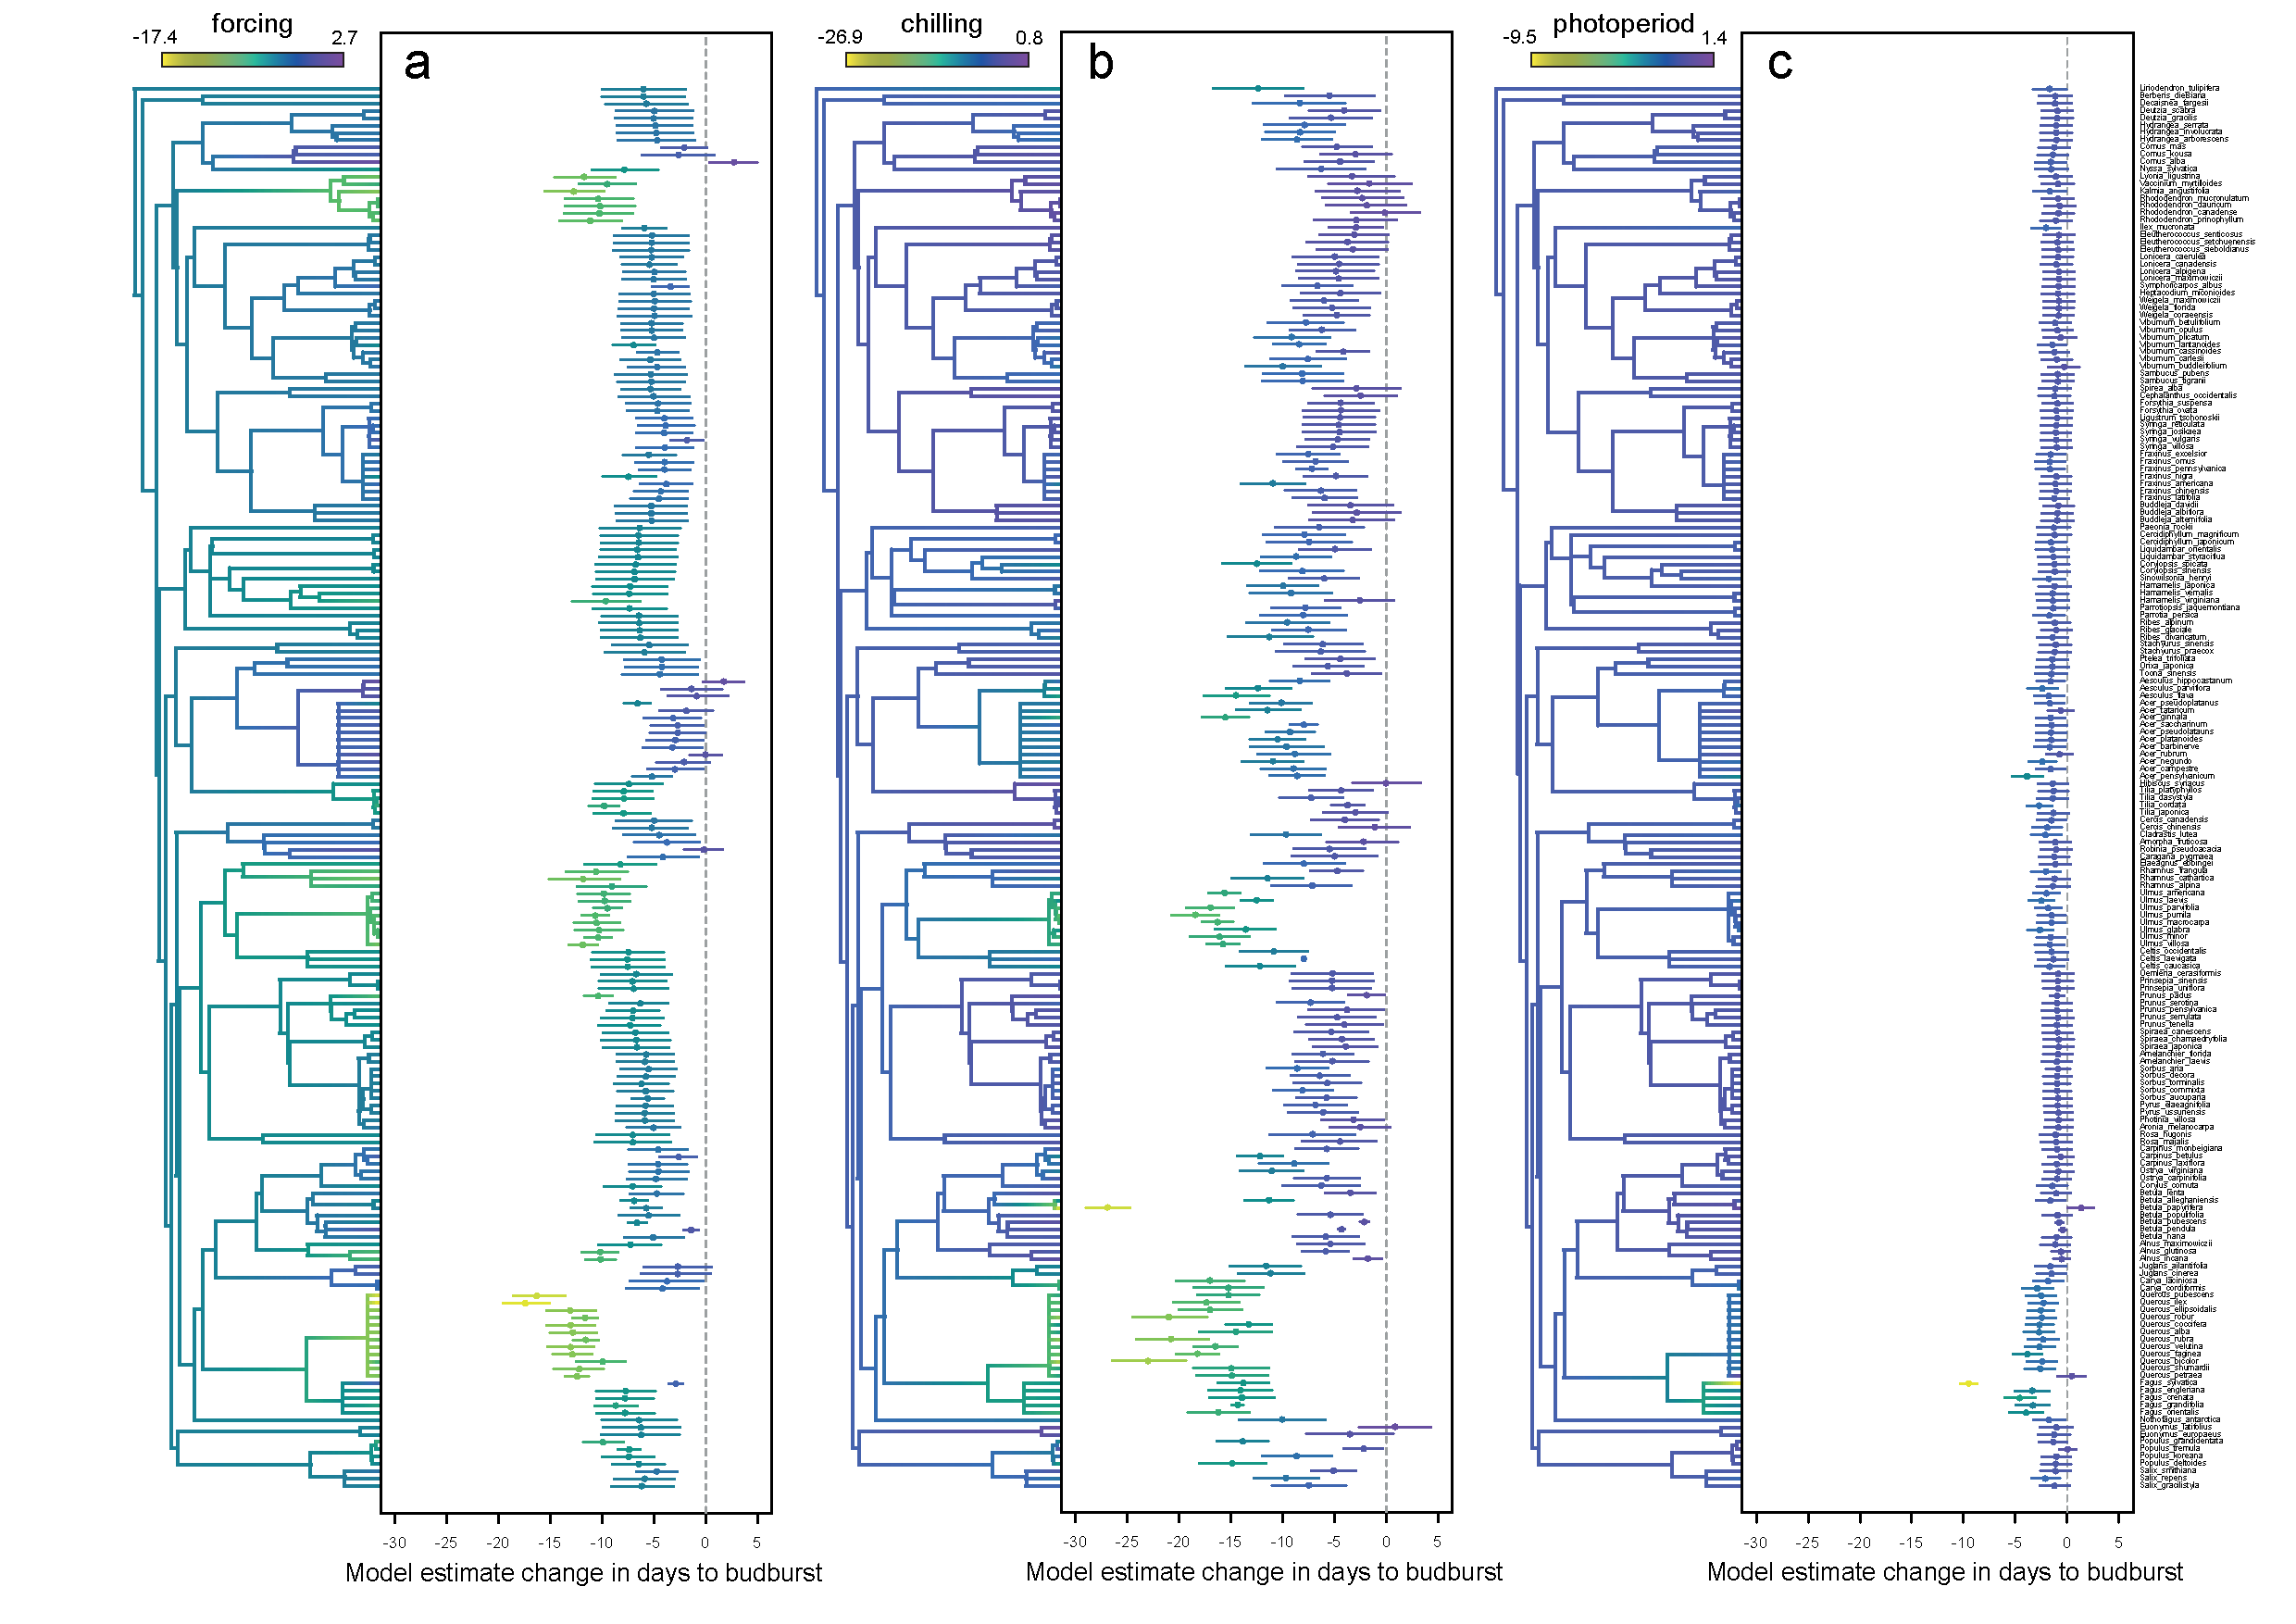
\includegraphics[width=16cm]{../../analyses/phylogeny/figures/muplot_phylo_allcue_angio.pdf}
  \caption{Phenological sensitivity to thee environmental cues, forcing (a), chilling (b) and photoperiod (c) measured in change in days to budburst per standardized unit (z-transformation) of the cues across 192 angiosperm species. The same phylogenetic tree is shown in each panel, colored acording to an estimation of ancestral character states, being the states at the tips the model slopes of our hierarchical phylogenetic model. Note that the color scale varies in each panel. Total tree depth is 81. My.}
  \label{fig:muplot_all}
  \end{center}
\end{figure}

\begin{figure} [H]
  \begin{center}
  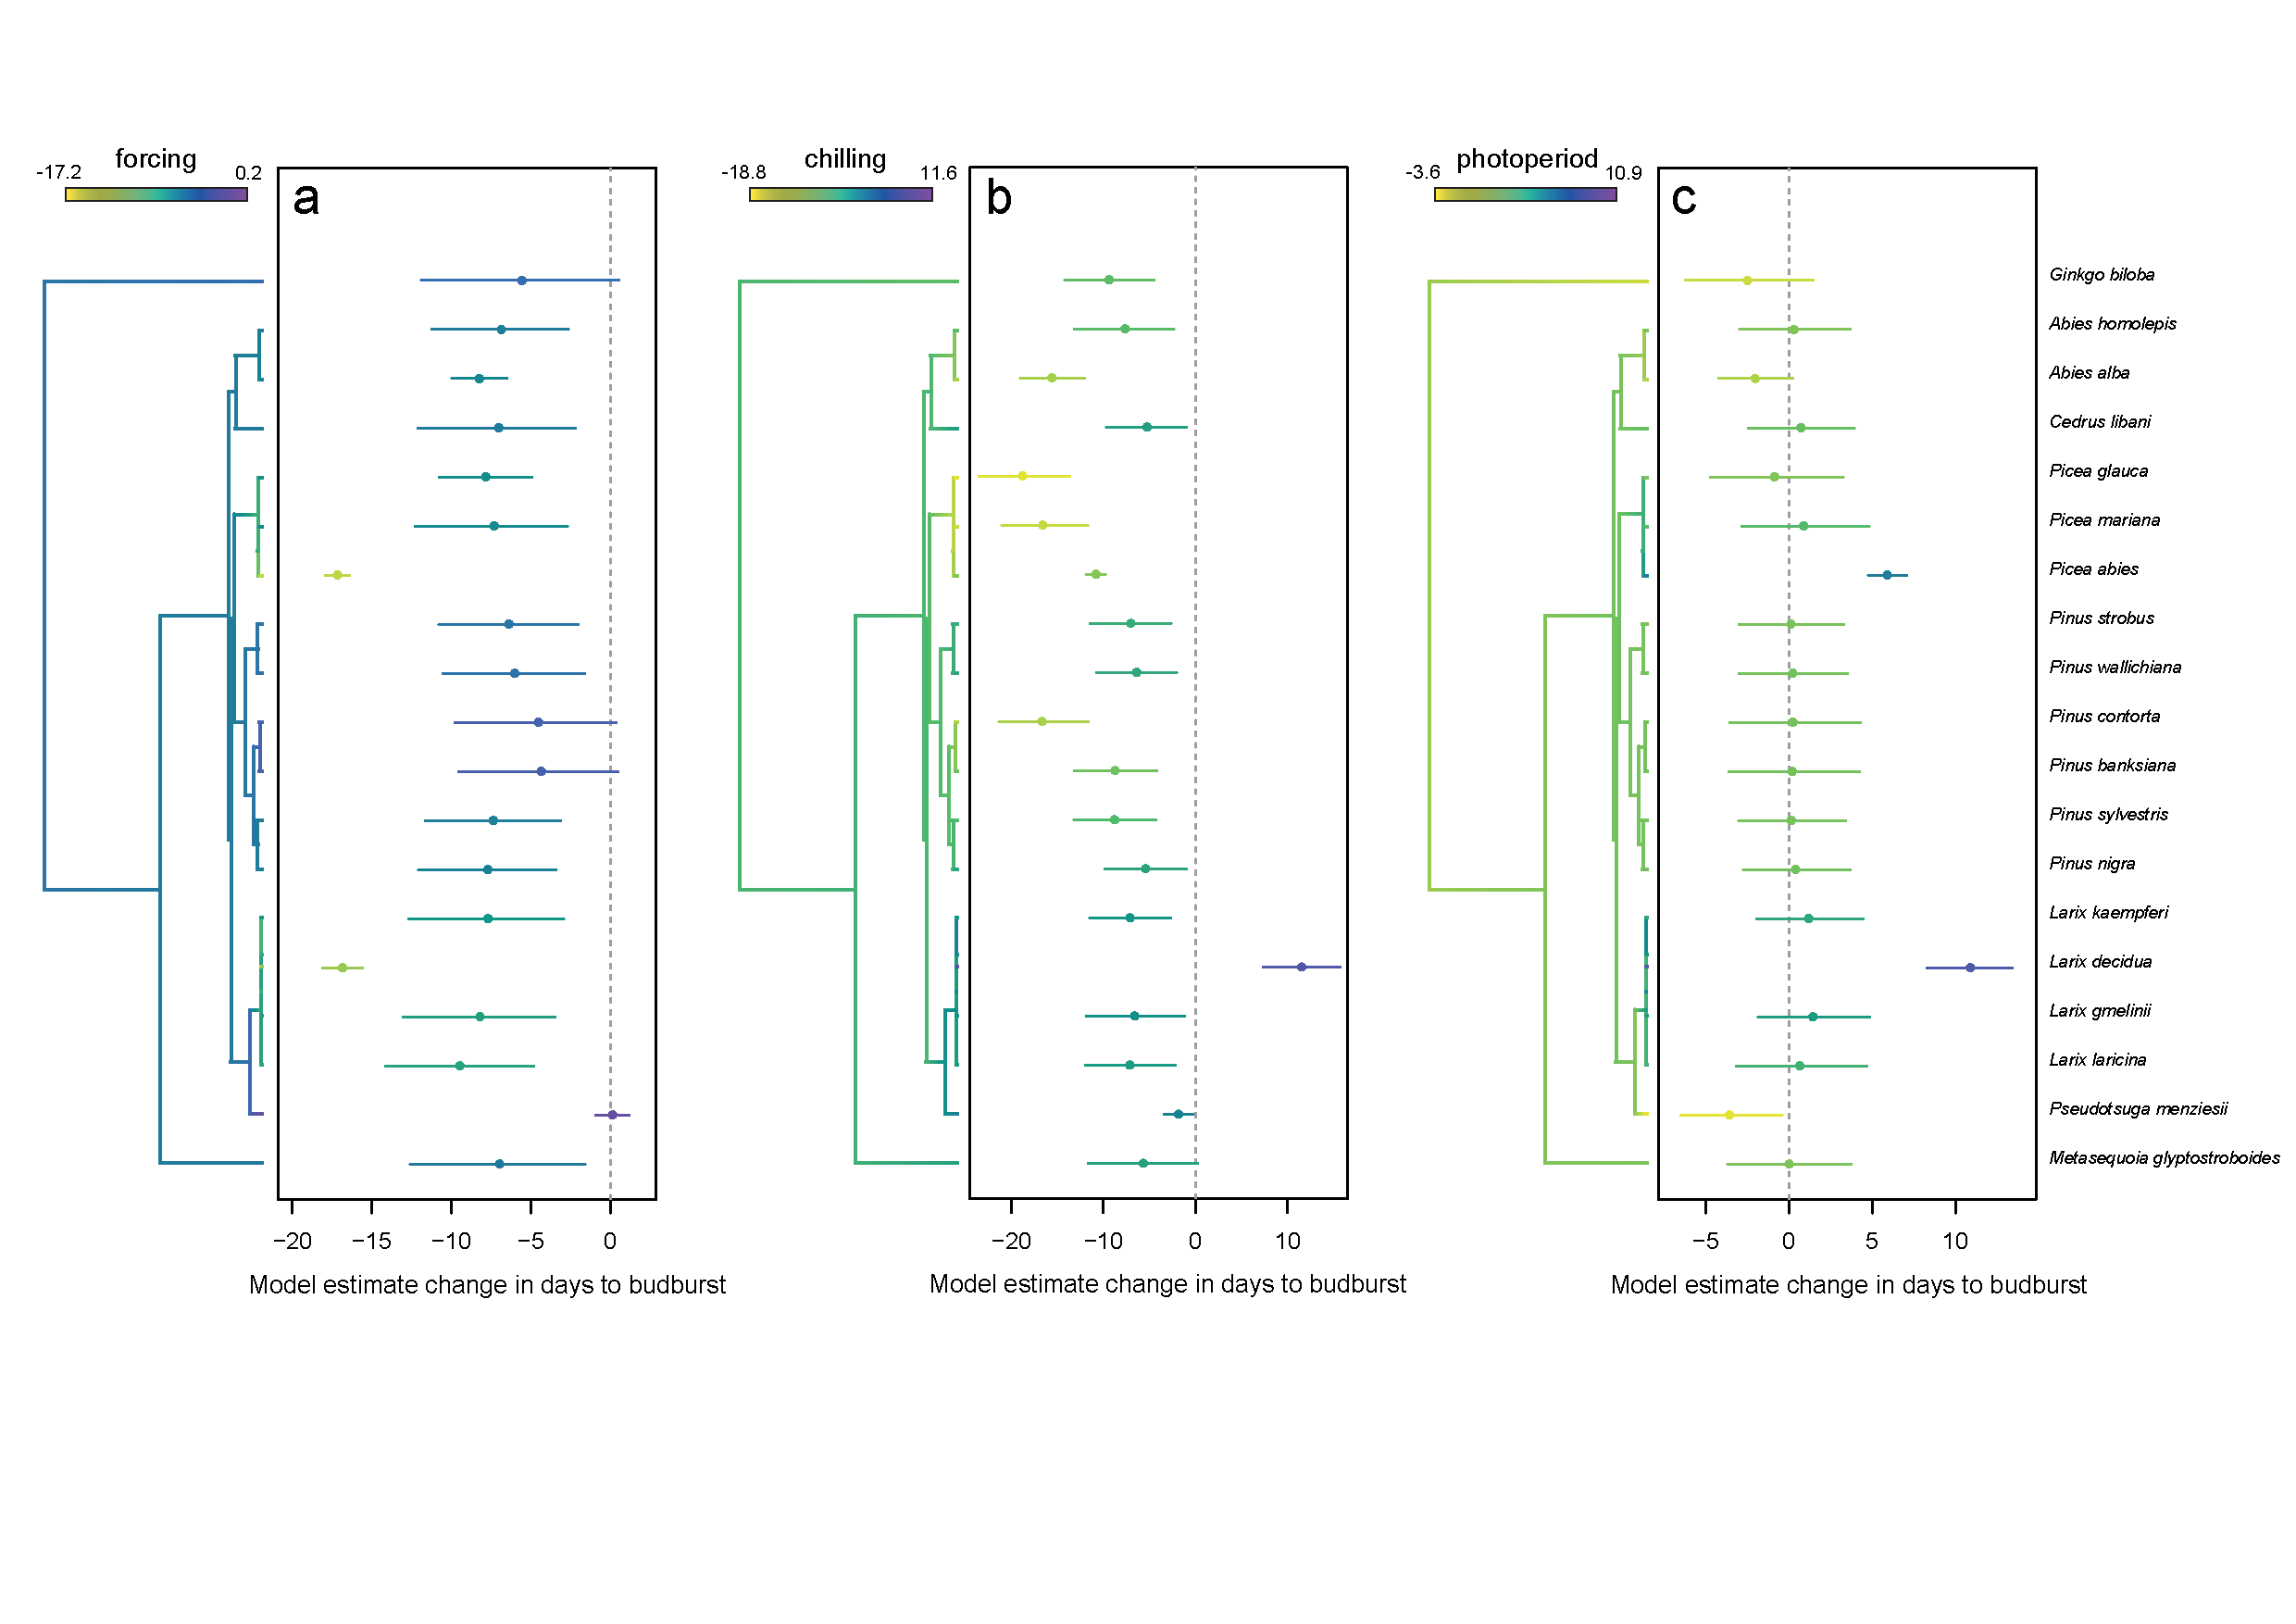
\includegraphics[width=16cm]{../../analyses/phylogeny/figures/Fig1b_phylo_muplots_gymno.pdf}
  \caption{Phenological sensitivity to thee environmental cues, forcing (a), chilling (b) and photoperiod (c) measured in change in days to budburst per standardized unit (z-transformation) of the cues across 19 gymnosperm species. The same phylogenetic tree is shown in each panel, colored acording to an estimation of ancestral character states, being the states at the tips the model slopes of our hierarchical phylogenetic model. Note that the color scale varies in each panel. Total tree depth is 81. My.}
  \label{fig:muplot_allgymno}
  \end{center}
\end{figure}


\begin{figure} [H]
  \begin{center}
  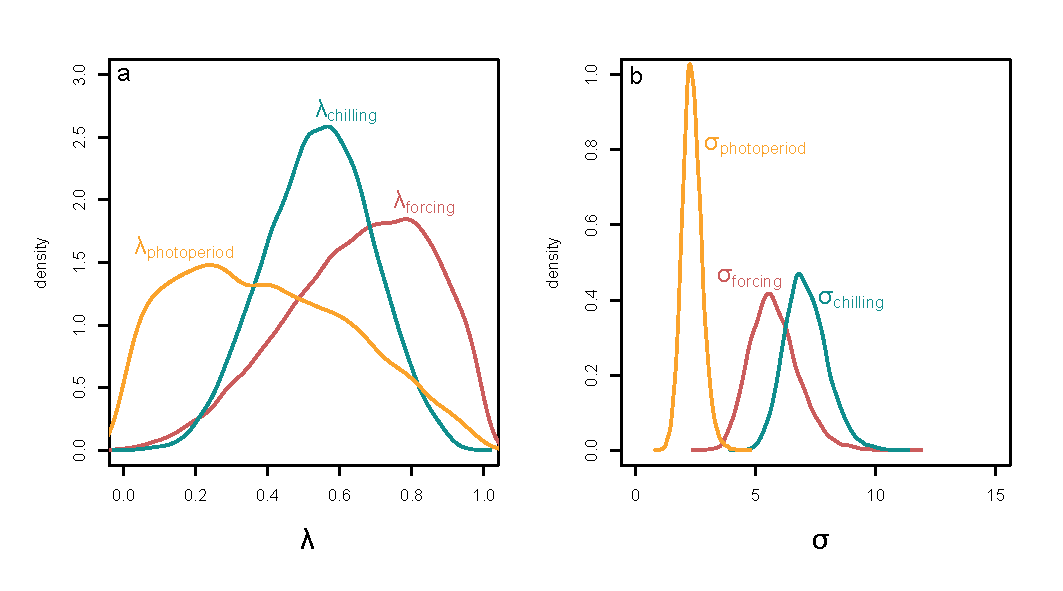
\includegraphics[width=14cm]{../../analyses/phylogeny/figures/Fig2_lambdas_sigmas.pdf}
  \caption{Density plots for the posterior distribution of phylogenetic signal measured by lambda for each cue included as a predictor in the model for angiosperms: forcing (red), chilling (blue),  photoperiod (orange) and for the model intercept (grey). Panels correspond to angiosperms (a-d) and gymnosperms (e-h). Note that lambda estimations corresponding to  panels c-d and g-h as they are constrained to be either equal zero or equal 1.}
  \label{fig:phylosig_all}
  \end{center}
\end{figure}

\begin{figure} [H]
  \begin{center}
  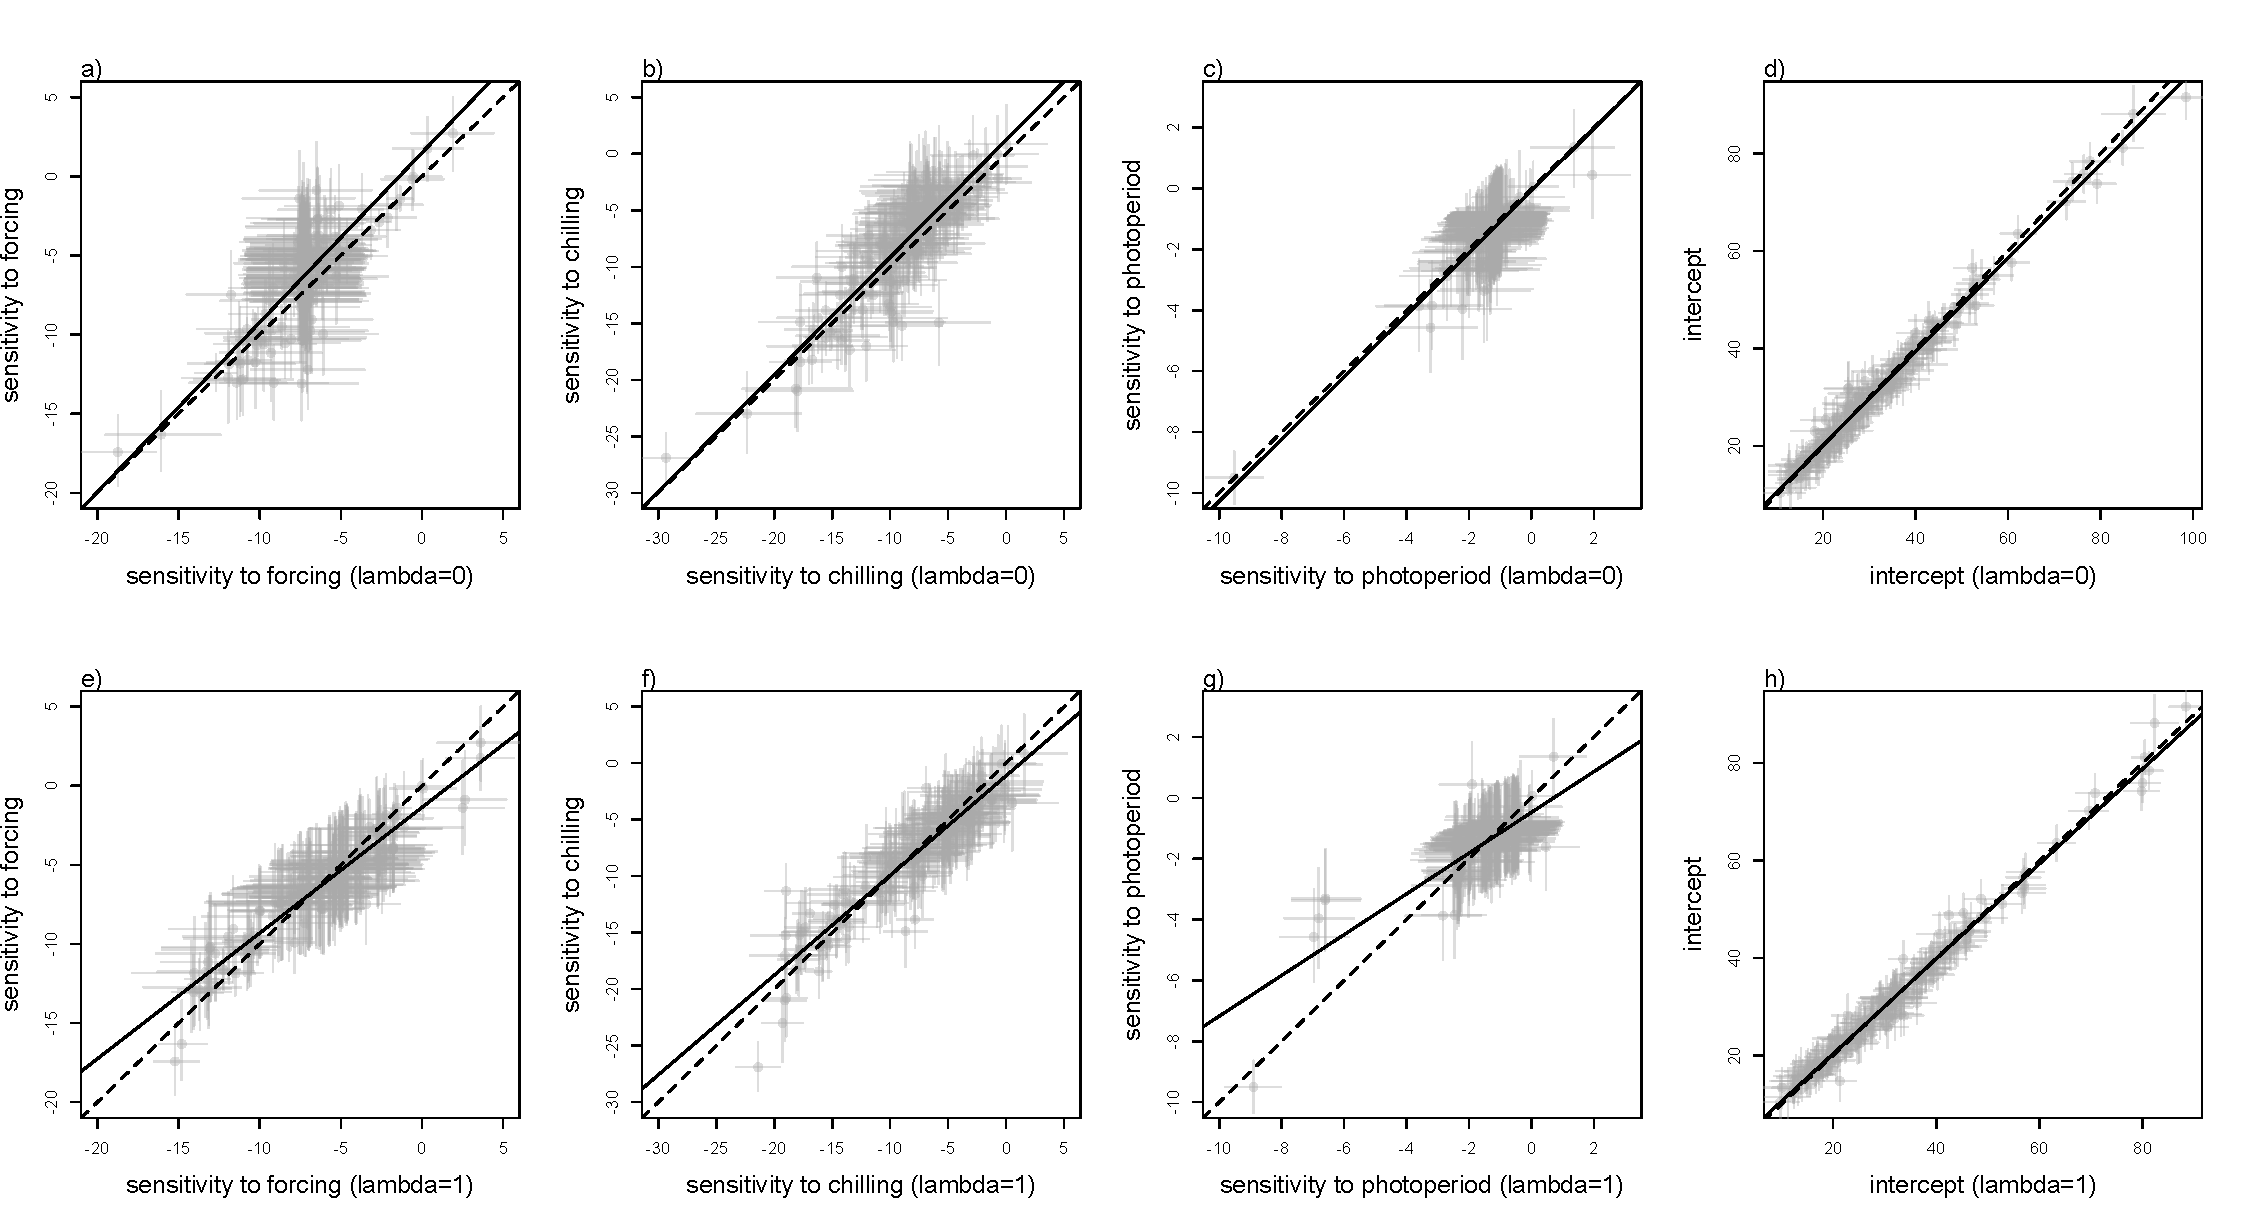
\includegraphics[width=14cm]{../../analyses/phylogeny/figures/Est_correls_vs_lamb01_angio.pdf}
  \caption{Correlations between model parameters as estimated by the full model and the models where lambda is constrained to be equal zero (upper row) or one (bottom row), for angiosperms. Panels correspond to sensitivity to forcing (a,e), to chilling (b,f), to photoperiod (c,g) and to model intercepts (d,h).}
  \label{fig:correls_angio}
  \end{center}
\end{figure}

\begin{figure} [H]
  \begin{center}
  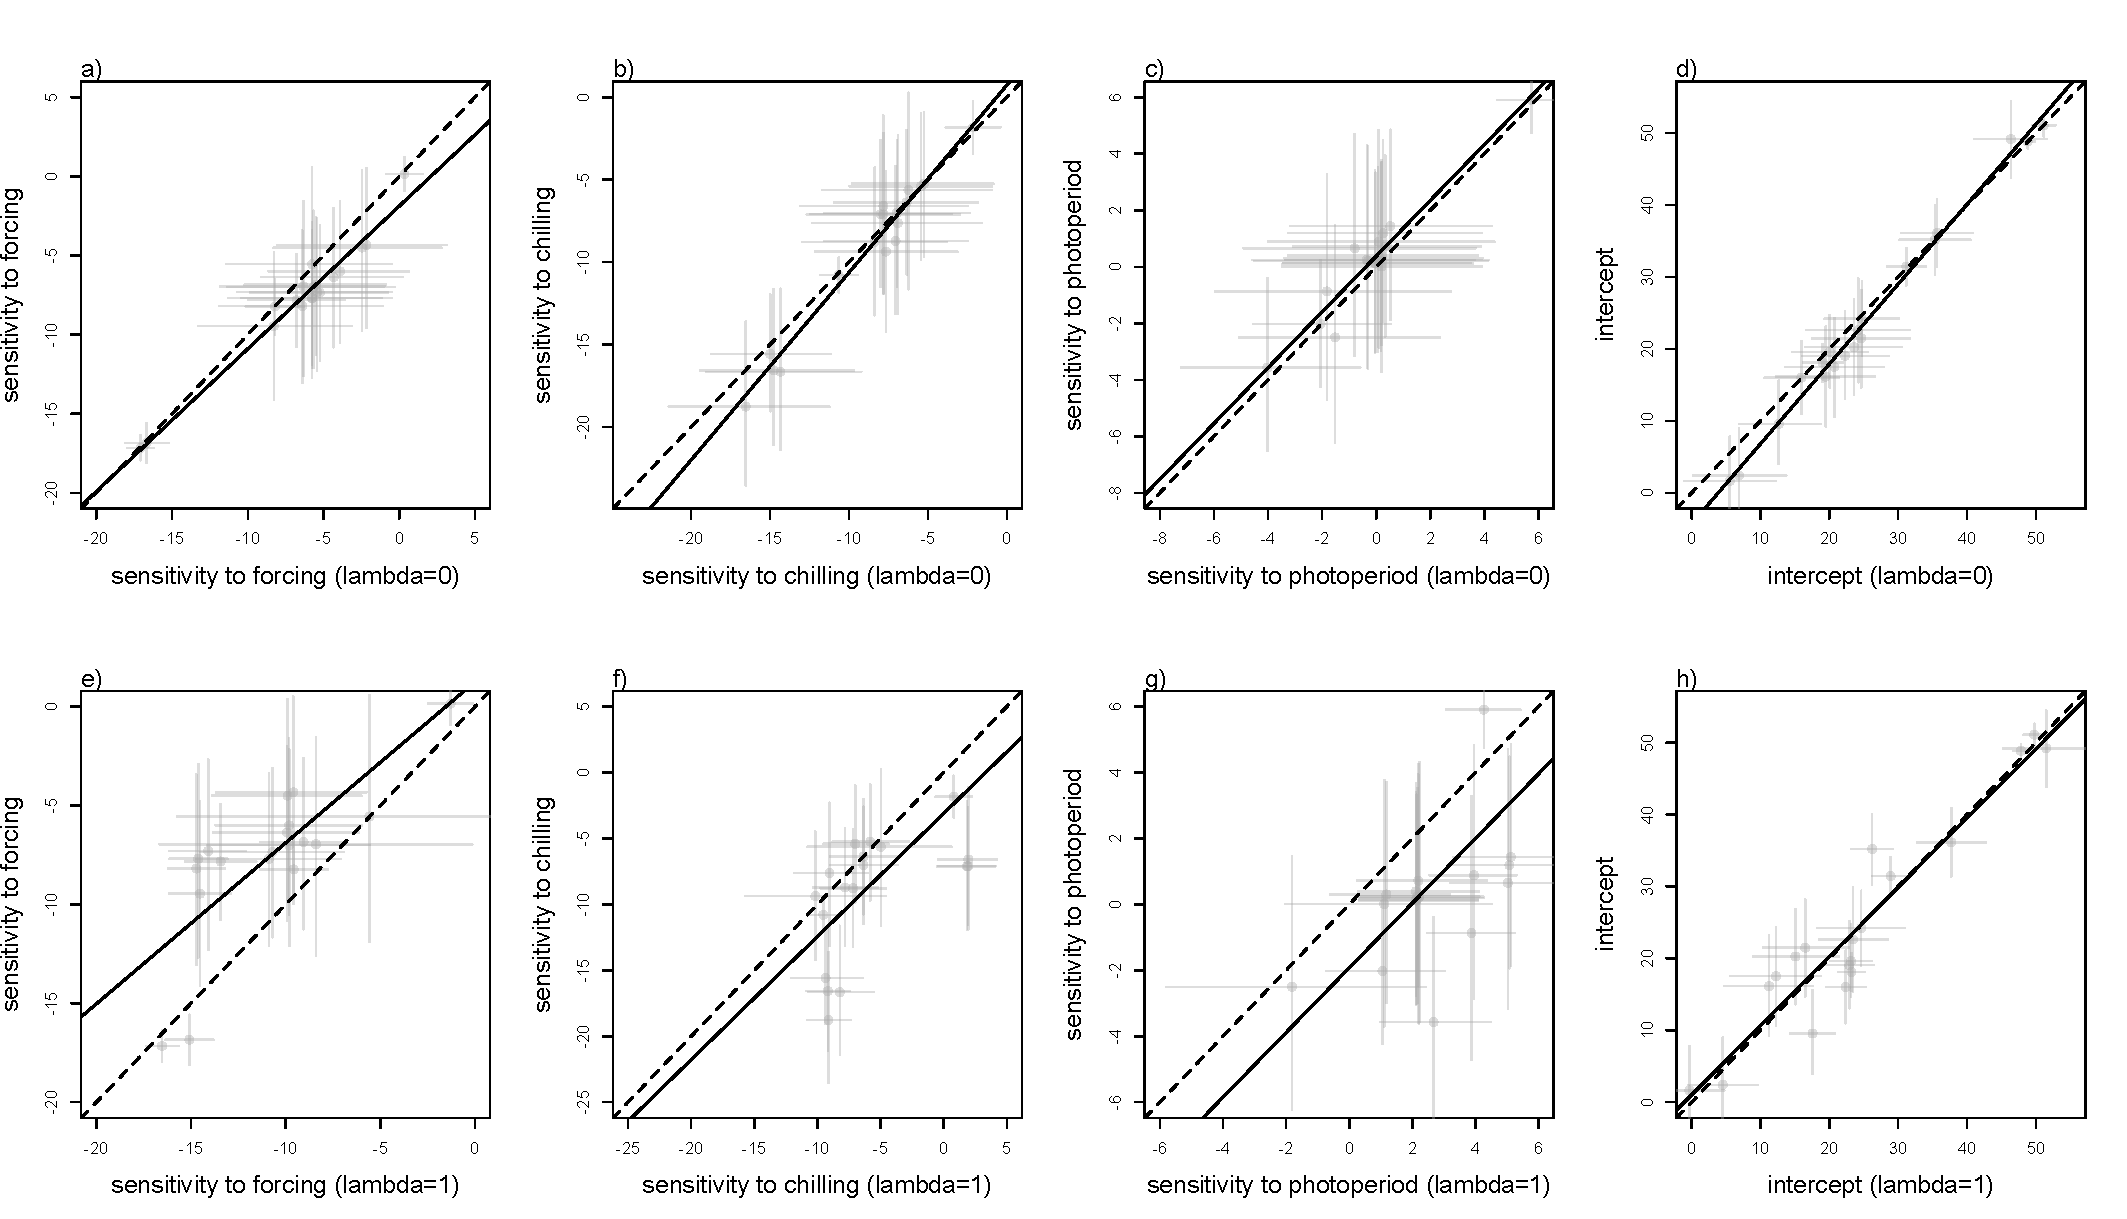
\includegraphics[width=14cm]{../../analyses/phylogeny/figures/Est_correls_vs_lamb01_gymno.pdf}
  \caption{Correlations between model parameters as estimated by the full model and the models where lambda is constrained to be equal zero (upper row) or one (bottom row), for gymnosperms. Panels correspond to sensitivity to forcing (a,e), to chilling (b,f), to photoperiod (c,g) and to model intercepts (d,h).}
  \label{fig:correls_gymno}
  \end{center}
\end{figure}



% IMC Mar21 - I'm guessing we are going to merge some of the tables below. TBD what we keep for the main text and what is sent to a supp.
\begin{table}[H]
\begin{center}
\caption{Full model parameters estimated for 192 angiosperm species.}
\begin{tabular}{@{}lcccccc@{}}
\toprule
\textbf{parameter}             & \multicolumn{1}{l}{\textbf{mean}} & \multicolumn{1}{l}{\textbf{sd}} & \multicolumn{1}{l}{\textbf{2.50\%}} & \multicolumn{1}{l}{\textbf{50\%}} & \multicolumn{1}{l}{\textbf{97.50\%}} & \multicolumn{1}{l}{\textbf{n\_eff}} \\ \midrule
$\mu_\alpha$                   & 30.57                             & 3.41                            & 23.68                               & 30.59                             & 37.14                                & 5031.19                             \\
$\mu_\beta_{forcing}$          & -5.84                             & 2.01                            & -9.72                               & -5.89                             & -1.79                                & 2374.73                             \\
$\mu_\beta_{chilling}$         & -7.19                             & 2.03                            & -11.15                              & -7.18                             & -3.18                                & 3694.93                             \\
$\mu_\beta_{photoperiod}$      & -1.37                             & 0.76                            & -2.92                               & -1.35                             & 0.14                                 & 1565.41                             \\
$\lambda_\alpha$               & 0.35                              & 0.10                            & 0.16                                & 0.34                              & 0.56                                 & 3416.51                             \\
$\lambda_\beta_{forcing}$      & 0.68                              & 0.20                            & 0.23                                & 0.71                              & 0.98                                 & 185.35                              \\
$\lambda_\beta_{chilling}$     & 0.56                              & 0.15                            & 0.25                                & 0.56                              & 0.83                                 & 738.57                              \\
$\lambda_\beta_{photoperiod}$  & 0.36                              & 0.24                            & 0.02                                & 0.33                              & 0.88                                 & 296.51                              \\
$\sigma_\alpha^2$              & 15.93                             & 1.17                            & 13.84                               & 15.85                             & 18.41                                & 2988.37                             \\
$\sigma_\beta^2_{forcing}$     & 5.84                              & 1.04                            & 4.03                                & 5.78                              & 8.15                                 & 502.74                              \\
$\sigma_\beta^2_{chilling}$    & 7.05                              & 0.87                            & 5.48                                & 7.02                              & 8.92                                 & 1026.77                             \\
$\sigma_\beta^2_{photoperiod}$ & 2.45                              & 0.41                            & 1.74                                & 2.42                              & 3.32                                 & 469.46                              \\
$\sigma_y^2$                   & 12.81                             & 0.18                            & 12.47                               & 12.80                             & 13.17                                & 4017.16                             \\ \bottomrule
\end{tabular}
\end{center}
\label{tab:modelanglamb}
\end{table}


\begin{table}[H]
 \begin{center}
\caption{Full model parameters estimated for 19 gymnosperm species.}
\begin{tabular}{@{}lcccccc@{}}
\toprule
\textbf{parameter}             & \multicolumn{1}{l}{\textbf{mean}} & \multicolumn{1}{l}{\textbf{sd}} & \multicolumn{1}{l}{\textbf{2.50\%}} & \multicolumn{1}{l}{\textbf{50\%}} & \multicolumn{1}{l}{\textbf{97.50\%}} & \multicolumn{1}{l}{\textbf{n\_eff}} \\ \midrule
$\mu_\alpha$                   & 25.75                             & 4.50                            & 16.88                               & 25.73                             & 34.73                                & 33151.86                            \\
$\mu_\beta_{forcing}$          & -5.92                             & 3.80                            & -12.97                              & -6.05                             & 1.90                                 & 16443.03                            \\
$\mu_\beta_{chilling}$         & -8.11                             & 3.63                            & -15.31                              & -8.09                             & -0.94                                & 21379.81                            \\
$\mu_\beta_{photoperiod}$      & -0.88                             & 3.33                            & -8.01                               & -0.67                             & 5.19                                 & 16301.93                            \\
$\lambda_\alpha$               & 0.47                              & 0.26                            & 0.02                                & 0.48                              & 0.90                                 & 15934.03                            \\
$\lambda_\beta_{forcing}$      & 0.36                              & 0.23                            & 0.02                                & 0.33                              & 0.84                                 & 14336.60                            \\
$\lambda_\beta_{chilling}$     & 0.32                              & 0.23                            & 0.01                                & 0.28                              & 0.82                                 & 13230.88                            \\
$\lambda_\beta_{photoperiod}$  & 0.37                              & 0.24                            & 0.02                                & 0.34                              & 0.88                                 & 11199.49                            \\
$\sigma_\alpha^2$              & 23.47                             & 6.20                            & 13.87                               & 22.59                             & 37.81                                & 18272.58                            \\
$\sigma_\beta^2_{forcing}$     & 8.89                              & 2.45                            & 4.96                                & 8.60                              & 14.51                                & 8126.51                             \\
$\sigma_\beta^2_{chilling}$    & 10.47                             & 2.66                            & 5.78                                & 10.30                             & 16.17                                & 8539.38                             \\
$\sigma_\beta^2_{photoperiod}$ & 7.18                              & 2.29                            & 3.29                                & 6.96                              & 12.25                                & 5625.69                             \\
$\sigma_y^2$                   & 15.81                             & 0.41                            & 15.04                               & 15.81                             & 16.63                                & 28640.16                            \\ \bottomrule
\end{tabular}
\end{center}
\label{tab:modelgymlamb}
\end{table}





\pagebreak
%\bibliographystyle{refs/bibstyles/amnat.bst}% 
%\bibliography{refs/phylorefs.bib}



\end{document}
